\section{Zeitplanung}
Für die Planung und Kontrolle des Projektfortschritts wurde pro Semester ein Zeitplan erstellt.
Die folgenden Gantt-Diagramme des 5. und 6. Semesters geben einen groben Überblick über diese.
Für das 5. Semester (siehe Abbildung \vref{fig:Gantt5}) wurden verschiedene Zeiträume aufgestellt, jedoch ohne inhaltliche Ziele.
Dem Zeitplan des 6. Semesters (siehe Abbildung \vref{fig:Gantt6}) wurden für die jeweiligen Zeitabschnitte inhaltliche Ziele hinzugefügt, wodurch der Fortschritt des Projekts besser kontrolliert werden konnte.

\begin{figure}[H]
	\centering 
	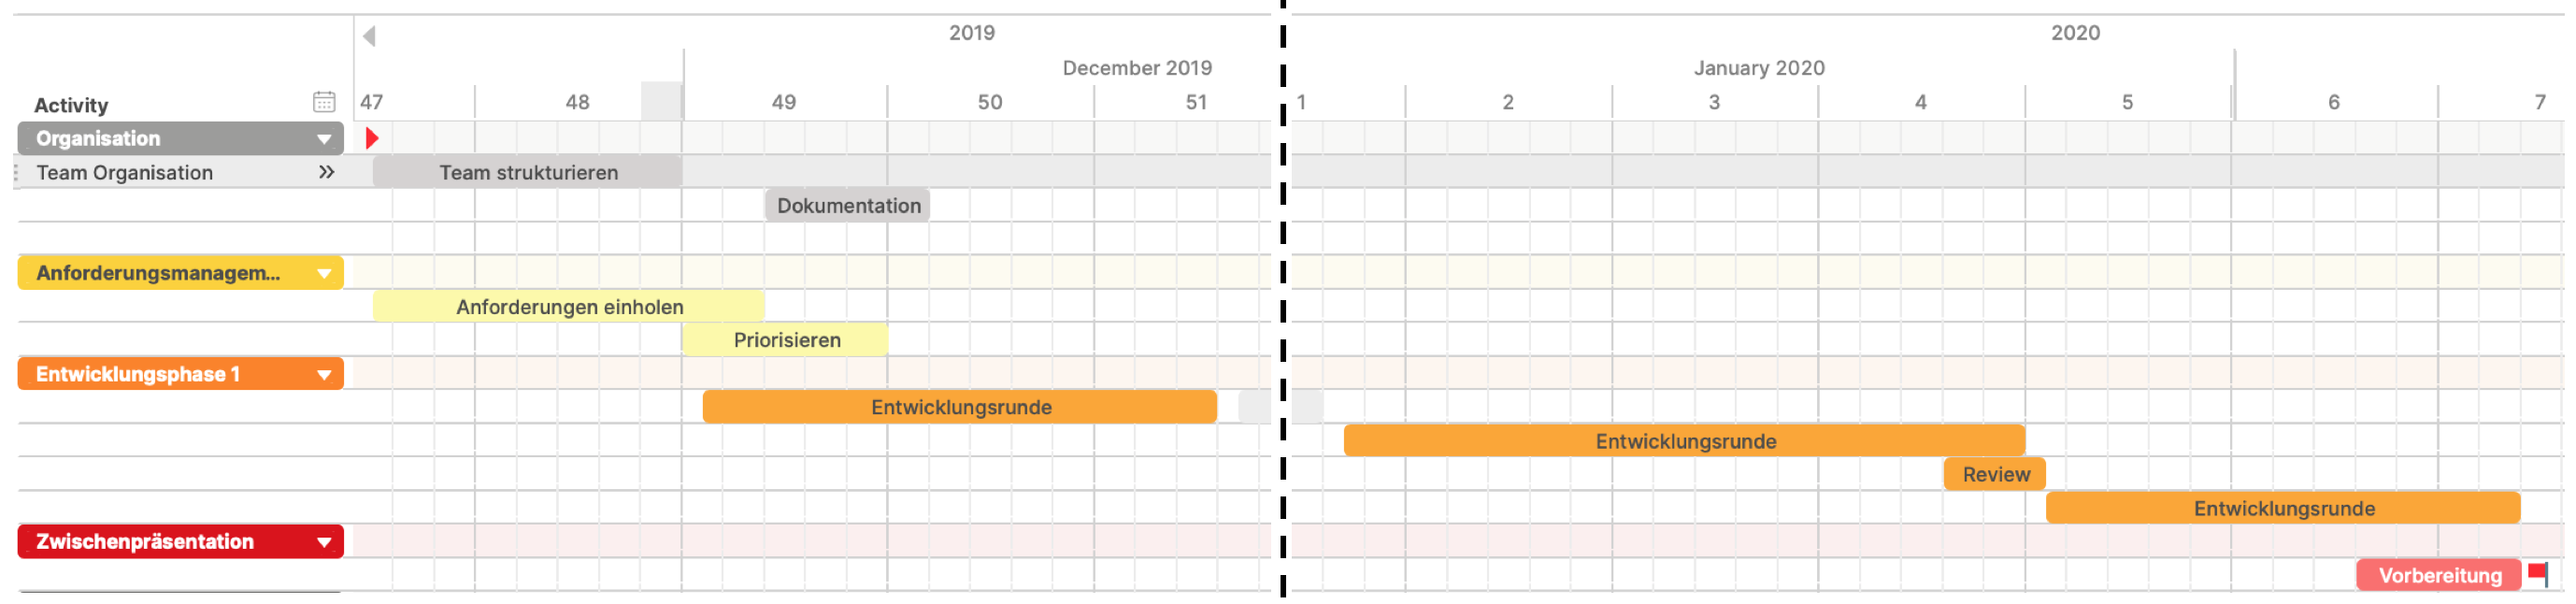
\includegraphics[width=\textwidth]{img/GanttSemester5.png}
	\captionsetup{format=hang}
	\caption[Grobe Übersicht Gantt-Diagramm Semester 5]{\label{fig:Gantt5}Grobe Übersicht Gantt-Diagramm Semester 5}
\end{figure}

\begin{figure}[H]
	\centering 
	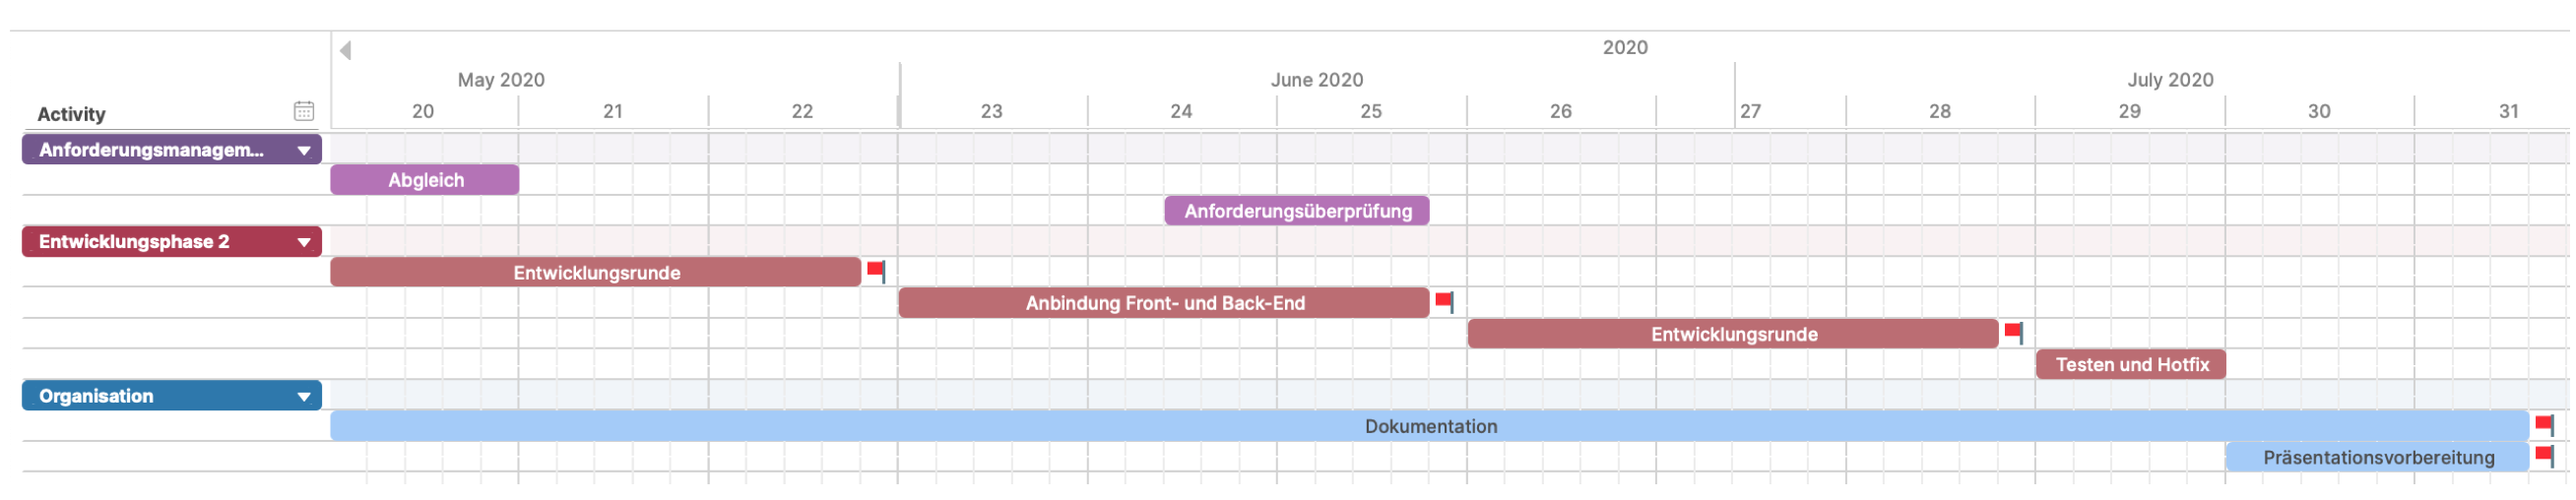
\includegraphics[width=\textwidth]{img/GanttSemester6.png}
	\captionsetup{format=hang}
	\caption[Grobe Übersicht Gantt-Diagramm Semester 6]{\label{fig:Gantt6}Grobe Übersicht Gantt-Diagramm Semester 6}
\end{figure}
